\documentclass[10pt]{article}
\usepackage{amsmath}
\usepackage{amssymb}
\usepackage{anysize}
\usepackage{listings}
\usepackage{graphicx}
\usepackage{xcolor}


\definecolor{Blue}{rgb}{0.2,0.2,0.9}
\definecolor{Green}{rgb}{0,0.6,0}
\definecolor{Gray}{rgb}{0.5,0.5,0.5}
\definecolor{Purple}{rgb}{0.58,0,0.82}
\definecolor{background}{rgb}{0.95,0.95,0.92}

\definecolor{bashtext}{rgb}{0.9,0.9,0.9}
\definecolor{bashbackground}{rgb}{0.3,0.3,0.3}

\lstdefinestyle{mystyle}{
    backgroundcolor=\color{background},   
    commentstyle=\color{Green},
    keywordstyle=\color{Blue},
    numberstyle=\tiny\color{Gray},
    stringstyle=\color{Purple},
    basicstyle=\ttfamily\footnotesize,
    breakatwhitespace=false,         
    breaklines=true,                 
    captionpos=b,                    
    keepspaces=true,                 
    numbers=left,                    
    numbersep=5pt,                  
    showspaces=false,                
    showstringspaces=false,
    showtabs=false,                  
    tabsize=2
}
\lstset{style=mystyle}

\newcommand{\ttt}{\texttt}

\newcommand{\tcpp}[1]{\hspace{10pt}\colorbox{background}{\textcolor{black}{\texttt{#1}}}}
\newcommand{\tbash}[1]{\hspace{10pt}\colorbox{bashbackground}{\textcolor{bashtext}{\texttt{\%~~#1}}}}
\newcommand{\troot}[1]{\hspace{10pt}\colorbox{bashbackground}{\textcolor{bashtext}{\texttt{root[~]~~#1}}}}

\setlength{\parindent}{0pt}

\title{Appunti Lezione 03}
\author{Lorenzo Visca}
\date{}

\begin{document}

\maketitle

\section{Interpretazione e compilazione di una macro}
L'istruzione presentata per utilizzare una macro in ROOT finora è stata:

\vspace{5pt}

\hspace{5pt}\troot{.L macro.C}

\vspace{5pt}

In questo modo la macro viene interpretata utilizzando l'interprete di ROOT (Cling).

L'interpretazione delle macro è utile per programmi molto leggeri, perché non prevede una fase di compilazione;
tuttavia per programmi più complessi l'interpretazione diventa lenta: è quindi consigliato compilare la macro, per cui la compilazione è inizialmente più lenta ma in compenso l'esecuzione è estremamente rapida.

NOTA: il compilatore è più “severo" dell'interprete, è quindi comunque consigliato compilare le macro in modo da individuare eventuali errori “soft" che l'interprete non segnala.

Per compilare una macro, le istruzioni sono:

\vspace{5pt}

\hspace{5pt}\troot{.L macro.C+}

\vspace{5pt}

Oppure:

\vspace{5pt}

\hspace{5pt}\troot{.L macro.C++}

\vspace{5pt}

La differenza tra \ttt{+} e \ttt{++} è che la prima opzione compila la macro solo se è stata modificata dopo l'ultima compilazione, mentre la seconda forza la ricompilazione della macro anche se non è stata modificata.
Questa seconda opzione è utile ad esempio quando si fa un upgrade di ROOT, del compilatore o del sistema operativo.

Quando una macro viene compilata vengono generati alcuni file:

\begin{itemize}
    \item un file \ttt{.d} che contiene le dipendenze della macro (ad esempio, se la macro include altre librerie);
    \item un file \ttt{.so} (su Linux) o \ttt{.dll} (su Windows) che contiene il codice compilato;
    \item un file \ttt{.pcm} che contiene altre informazioni di compilazione utilizzate dal sistema per velocizzare l'esecuzione.
\end{itemize}


\newpage
\section{Apertura di un file ROOT}
Una volta creato un file ROOT (ad esempio contenente un istogramma come quello creato in \ttt{ioexample2.C}), è possibile accedervi in due modi:

\begin{itemize}
    \item tramite il browser di ROOT, che fornisce un'interfaccia grafica per la navigazione dei file e la possibilità di effettuare varie azioni sul loro contenuto (per accedere all'istogramma fare doppio click sul nome del TFile che lo contiene);
        
        \vspace{5pt}

        \troot{new TBrowser()}

        \vspace{5pt}
    
        \begin{center}
            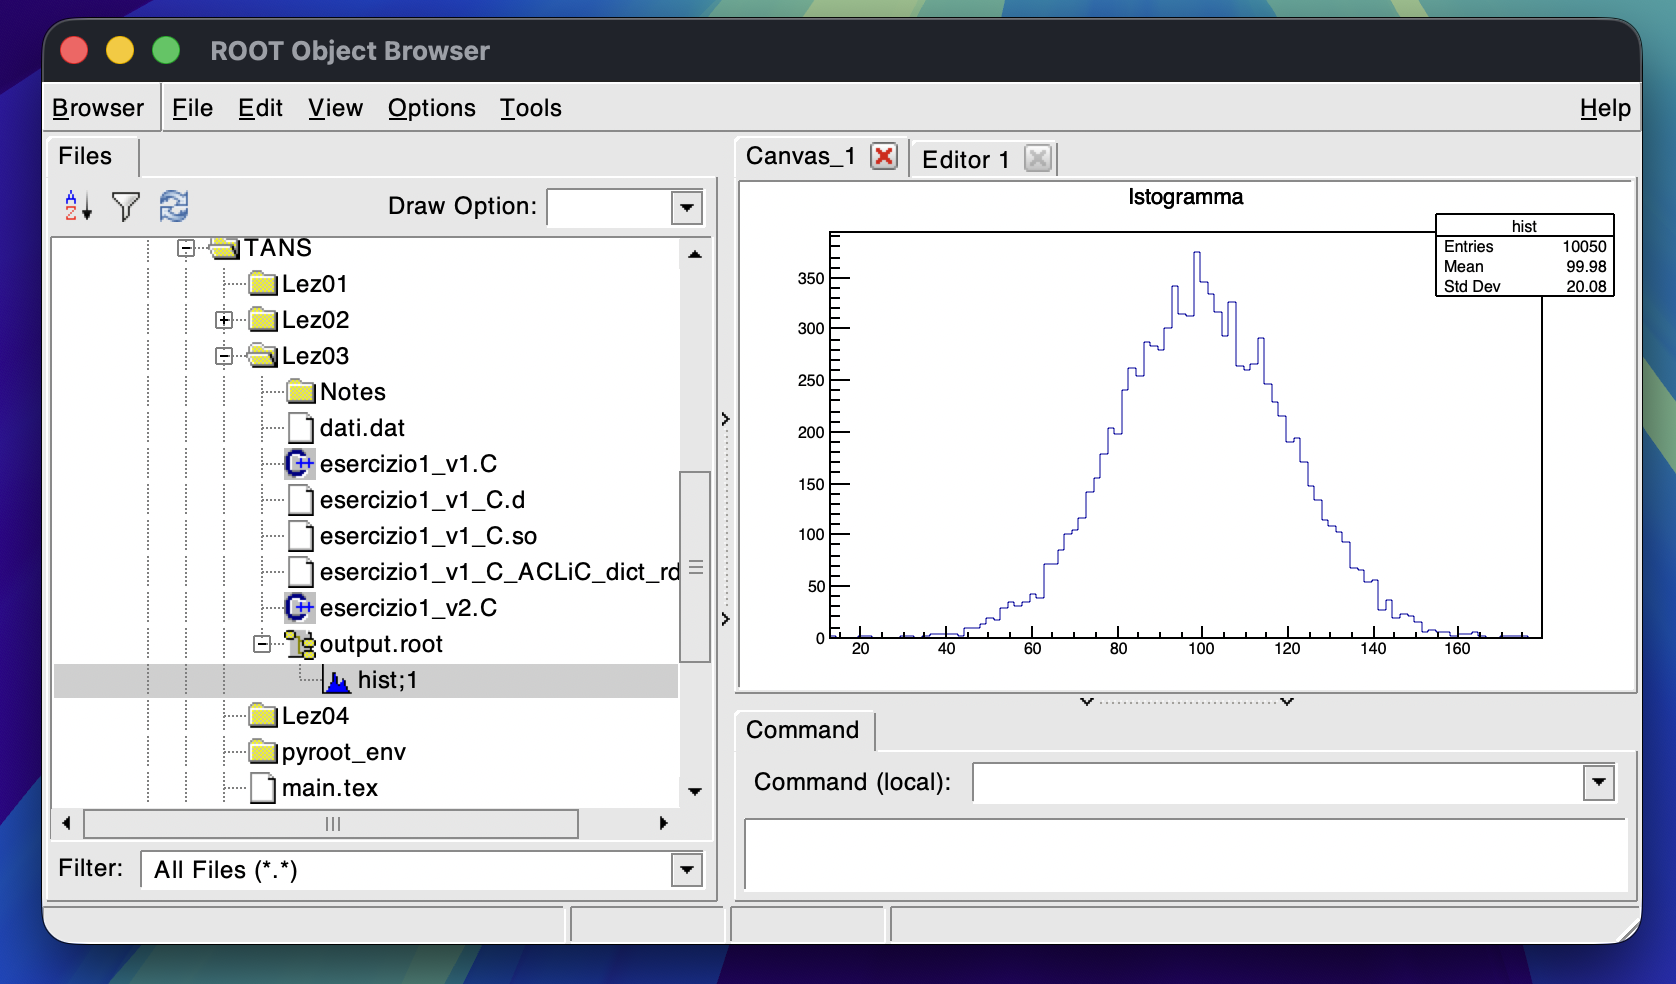
\includegraphics[width=0.6\linewidth]{Browser.png}
        \end{center}

    \item richiamando il file all'interno di un'altra macro:
    
        \tcpp{TFile *myfile = new TFile("output.root");}

        \tcpp{TH1D *myhist = (TH1D*) myfile->Get("hist");}

        \tcpp{myhist->Draw();}

        Il comando \ttt{Get} prende l'oggetto il cui nome ricordato da ROOT è \ttt{"hist"}, ovvero il primo argomento dato al costruttore di \ttt{TH1D} nella macro che l'ha creato.

        Normalmente \ttt{Get} restituisce un puntatore di tipo \ttt{TObject}, che è la classe base di tutte le classi in ROOT. Per interpretare l'oggetto come istogramma è quindi necessario effettuare un cast esplicito con \ttt{(TH1D*)}.

        \vspace{5pt}

        Strutturando il codice in questo modo l'istogramma rimane linkato a \ttt{myfile}, quindi quando esso viene chiuso non è più possibile accedere all'istogramma. Per slegare l'istogramma dal file, si può usare il comando:

        \tcpp{hh->SetDirectory(NULL);}

\end{itemize}


\newpage

\section{Esercizio}

Realizzare un programma analogo a \ttt{ioexample2.C} che però non richieda di sapere a priori l'intervallo in cui sono distribuiti i dati.
Il programma non deve richiedere a priori il numero di dati presenti nel file di input.

\section{Soluzione: descrizione}
Codici di riferimento: \ttt{esercizio1\_v1.C}\hspace{10pt}\ttt{esercizio1\_v2.C} \vspace{10pt}

Il problema è affrontabile in due modi:
\begin{enumerate}
    \item (\ttt{esercizio1\_v1.C}) Il file di input viene letto due volte: la prima volta si conta il numero di dati e si tiene traccia del minimo e del massimo, la seconda volta si riempie l'istogramma.
        Questo metodo è vantaggioso dal punto di vista della memoria, in quanto non è necessario allocare un vettore per contenere i dati.
        Tuttavia, è svantaggioso in termini di tempo, in quanto le operazioni di lettura da file sono piuttosto lente e in questo caso tale operazione viene eseguita due volte.
    \item (\ttt{esercizio1\_v2.C}) Il file di input viene letto una sola volta, durante la quale oltre a contare il numero di dati e tenere traccia del minimo e del massimo, si memorizzano i dati in un vettore.
        Questo metodo è vantaggioso in termini di tempo, in quanto il file viene letto una sola volta, tuttavia è svantaggioso in termini di memoria, in quanto è necessario allocare un vettore per contenere i dati.
        Inoltre, non è possibile sapere a priori quanto grande deve essere il vettore, quindi si utilizza un vettore dinamico della classe (\ttt{std::vector}).
\end{enumerate}

\section{Soluzione: extra}
Codice di riferimento: \ttt{esercizio1\_v2.C} \vspace{10pt}

In questo esempio viene data la possibilità di specificare il numero massimo di dati da leggere come argomento opzionale della funzione.
Per definire un argomento opzionale, è sufficiente assegnargli un valore di default nella dichiarazione della funzione:

    \tcpp{void esercizio1\_v2(..., const unsigned int limit = 100000)}

In questo modo, se la funzione viene chiamata con solo due argomenti, l'argomento \ttt{limit} assumerà il valore di default \ttt{100000}.
Se invece la funzione viene chiamata con tre argomenti, il terzo argomento assumerà il valore passato nella chiamata.

\newpage
\section{Soluzione: codici}

\subsection{esercizio1\_v1.C}
\lstinputlisting[language=C++]{../esercizio1_v1.C}

\newpage

\subsection{esercizio1\_v2.C}
\lstinputlisting[language=C++]{../esercizio1_v2.C}

\end{document}